\documentclass[main.tex]{subfiles}
\begin{document}

\section{Fusion}

For all the methods we tried, each road is detected by a lot of different chains all covering only a portion of the road, and some chains overlap. This means that we do find all the road in the end (at least for the ones we don't have trouble detecting), but it would be preferable to have only one very long chain covering all the road. Since we can not do this simply with the detection, the idea would be to fuse the chains we find together, to end up with this better result. It would also help to have less chains if we want to use them afterwards for other calculation.

This is why we implemented the function \texttt{fuse\_all\_chains}. It can be used after the Triplets or the Follow line methods. It works by testing each couple of chains, so it is best to use it for an already optimized method that does not make a lot of noise and thus too many chains, even if it is particularly good in these situations to fuse the chains in order to have less of them. For each couple of chains, they will be fused if they are in a similar direction, and if their extremities are close enough. This means we use two parameters : \textit{fusion\_angle\_thresh} which is the maximum angle accepted between the directions, and \textit{fusion\_dist\_thresh} which is the maximum distance between the extremities. 

This method has been tested and used a little, but we ended up concentrating on improving the methods in themselves instead, so we did not perfect it and can not say which parameters would be the best to use. It would probably be good to work on it again because it does help especially with the methods giving very short chains.

% pictures ?

\section{Error function}

In order to have a way to compare our methods and be able to say if they are giving "good" or "bad" results, we decided to create an error function. This function simply compares the length (in km) of the chains found, to the real length of roads in France. The roads that we try to detect  with our methods are the main ones: highways, national roads, and train tracks. However, the reference value we use for the real roads length comprises these roads and adds the departmental roads. This is because every methods we have has a lot of noise, especially in the cities, and this compensates it. Meaning, the length we detect is in general closer to the value counting the departmental roads, and if we did not count it we would always have a very big error even though visually the results are very good. 

The data for the length of the roads was found on \href{https://www.insee.fr/fr/statistiques/2012705#tableau-TCRD_076_tab1_departements}{L'INSEE} from 2023, and for the train tracks it is still from \href{https://www.observatoire-des-territoires.gouv.fr/longueur-des-lignes-ferroviaires-en-service}{L'Observatoire des Territoires} from 2010. However the first data-set has "departmental and communal roads" together, while we want to separate them to consider one of them and not the other. So we found the total length of the departmental roads on \href{https://fr.statista.com/statistiques/540868/longueur-routes-france-par-type/}{Statista}, but we won't be able to have this value per department.

Our error function returns the reference length, the detected length, the absolute error and the relative error. This last one is sometimes even above 100\% when we really have a lot of noise. 

\hfill

We then upgraded this function a little, since here we only have a global value, it does not take into account \textbf{where} we find the roads. In order to add a bit of this notion, we transformed the error into a score taking into account this relative error but also the standard deviation of the relative errors by department. This is to translate that we want each department to be detected just as well, we don't want to detect way too many roads in Paris and then none in the countryside for example. 

To calculate the errors by department, we used the same data-set from L'INSEE, but we could use only train tracks + highways + national and not departmental roads, which means the reference value is always much lower than the detected value and we have pretty high values. But since we don't use the values directly but their standard deviation, we still have a usable value. The score is thus calculated with $score = \alpha \times global\_rel\_err + \beta \times std\_rel\_err\_dep$. $\alpha$ and $\beta$ values were set after a few tests to $0.97$ and $0.03$, as otherwise there was too much importance given to the standard deviation and results where we found no roads at all were considered very good (and sometimes the best) because even if they have a very high global error, each department is detected just as well so the deviation is 0. 


\section{Follow line by density of stations}

This method is the one that gave the best results, which is why these next upgrades were only applied to it. However they could be easily applied to our other methods as well.

\subsection{Parameters optimization}

A problem we have with most of the methods is the amount of parameters to set. Most of them have been tested with different values to try and find the best result, but we can not test every set of parameters, and changing one of them influences the others. It is thus very complicated to decide which values to use. However, now that we have an error function, we can assume that a set of parameters giving a result that minimizes the error would be ideal and giving the best result. In reality, our error function does not perfectly take into account the geography of where we found our roads, so we might encounter results with so much noise somewhere that the error is low even though we did not detect roads anywhere else. But most of the time using this error function is good to determine if a result is better than another. 

The first parameter for which it was hard to set a value is the radius for the density calculation. Indeed we used approximately the radius of Ile de France as it is the largest most dense area of the map, so it seemed to make sense. But actually maybe it would be better to use another radius, in which case it is really hard to determine which value it should be. This is why we tried different values for the radius to see which one minimized the error, without changing the other parameters. However, we did do this for different values of the distance parameter, and every time the final result was different. This shows that every parameter influences the others a lot, and we cannot dissociate them. This is why we decided to optimize every parameter at the same time.

% Make sure it was the distance parameters ! And maybe put the pictures that I had different results with different distances ??

In order to optimize the parameters, we used the python library \texttt{skopt} and the function \texttt{gp\_minimize}. This function works by giving it a space of parameters, and then chooses in this space different set of parameters to minimize our error function. It starts with a few iterations where it chooses the points in the space randomly, and then uses these points and their result to optimize for the rest of the iterations. This means we have to firstly create the space by setting an interval in which each of the parameters have to be chosen, and then, we have to set the total number of iterations of the optimization and the number of random search iterations at the start. We also set the random seed, which most of the time was at 43, but we sometimes changed it and got different (better or worse) results. This is because our method takes a lot of time so we can't do a lot more than 20 iterations and of course it is hard to find a perfect result with so little iterations when we have so many parameters. For the same reason, we started with very large intervals for our parameters to be sure not to miss a result and not have any bias, but then after a few runs reduced the intervals according to the results we had so as to reduce the searching space and find better results. We also set the intervals to be discrete for the same reasons.

\textbf{Parameters intervals : }
\begin{itemize}
    \item r\_density : 20 000 - 60 000, after a few tests most of the time the optimal result stays around 40 000.
    \item n\_neighbors : 10 - 20 after a few tests. It would not make sense that the next station of the road is further than the 20th closest neighbor. 
    \item n\_directions : 2 - 5. According to the tests done prior.
    \item angle\_tol : 0 - 15. If we set it too high we lose the point of going into different directions because we may miss some. We can also let it be 0 because this parameter might be useless.
    \item dist\_min :  1 - 400 after a few tests and considering the minimum distance between two points.
    \item dist\_max :  5500 - 8000 after a few tests and considering the mean distance between two points. Larger intervals were tested, but the optimal result was always in this interval, and when the program tests with very high distances it takes a lot more time to compute. Seeing how it does not give better results with higher distances and already takes a lot of time here, it is mostly useless to go higher than 8000.
    \item angle\_min : 15 - 80. One of the hardest parameters to estimate, but doesn't influences the result this much. Although most of the time the optimal result keeps it pretty high.
    \item angle\_max : 70 - 90 to really give the least constraint to finding roads in the countryside, and according to the previous results. 
    \item min\_len:  15 - 45. When going higher, usually the optimal result does have higher roads, but visually the results are not as good. Thus here "forcing" the value to be lower than 45 helps having control on the final result. 
\end{itemize}


\subsection{Detection without cities}

Seeing how all of our methods create a lot of noise in the cities, detecting so many roads in them, we tried simply removing the stations in the cities. Indeed, there are no important roads directly in the cities, so we don't want to detect anything in them. To remove the stations in the cities, we simply use the mean distance to the nearest neighbors, if it is lower that a value, then we remove the station. This is equivalent to removing the stations in the most dense areas. Once these stations were removed, we simply apply our method of choice. Here it is the Follow line by density method, but we also tried with the simple Follow line method and it works similarly.

We immediately tried it in the optimization program, so that we wouldn't have to do multiple tests ourselves to find the best parameters but instead would just let the program do it. We did have to think about modifying the intervals a bit, for example maybe the minimum distance and angle could be higher now since the denser areas would not be the same ones, but in the end the intervals did not change much because there are still some very dense areas and anyways the program finds the best parameter. What we did change is the reference value for the error. Since there isn't all the noise in the cities anymore, we don't need to compensate with the departmental roads length, and removed it from our reference length.

\begin{figure}[H]
    \centering
    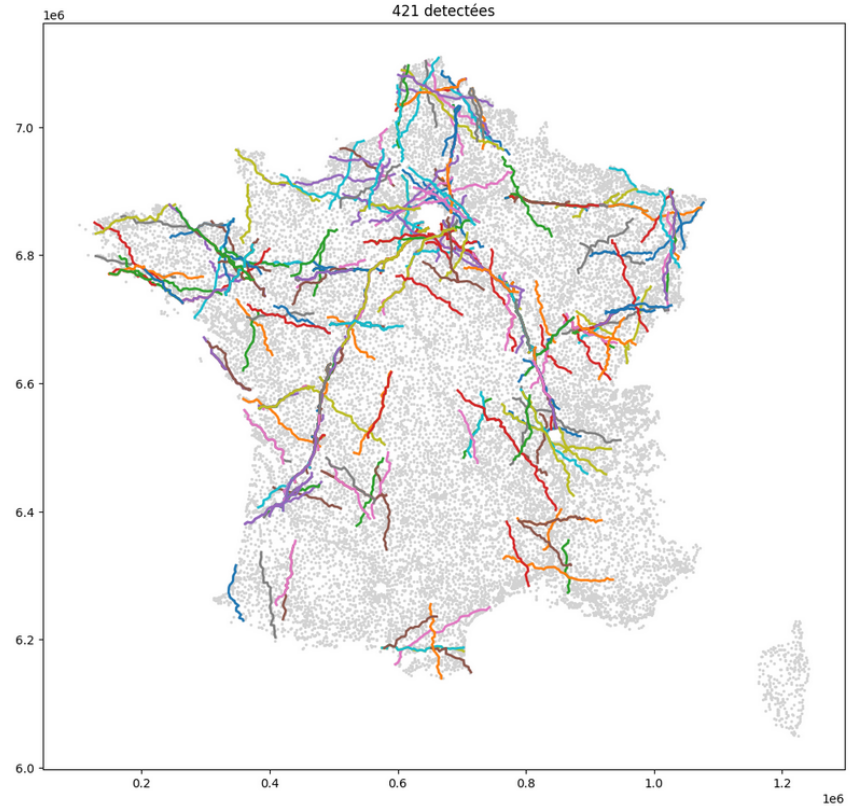
\includegraphics[width=0.7\textwidth]{Images/Res_Sansvilles.png}
    \caption{Detection without cities - Follow line by stations density}
\end{figure}

In the end, the results were pretty similar to what we had before. We still detect the same roads and have trouble detecting the same others, although maybe there are more roads that we have trouble detecting. So this solution might be a good idea to look into and improve, as once again it is interesting to obtain less chains in the end if we want to do something with them afterwards, but it is not necessarily giving better results. We can also consider that it is not a bad thing that we detect so many roads in the city, because if we think about our end goal being that the stations along a road are going to be neighbors, then in cities if we detect roads it means these stations are very close and would probably be considered as neighbors in the end anyways. 


\subsection{Non linear adjustment of parameters}

\begin{figure}[H]
    \centering
    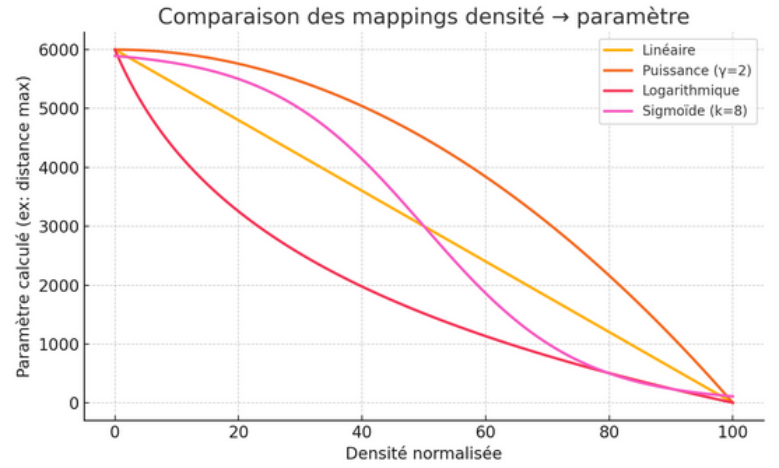
\includegraphics[width=0.7\textwidth]{Images/Nonlin_graph.png}
    \caption{Curves comparison of different transformations}
\end{figure}

We also looked into how the parameters were adjusted according to the density. For the moment, the distance and angle parameters are adjusted to the density with a linear transformation. However, we could try using other transformations. We tried an exponential transformation (power), a logarithmic one, and a sigmoïd one. Each of these transformation will also depend on one new factor parameter. However, after testing all of them on only one region and then on France, we realize that there really is a very small difference, even when trying different factors values for them. Hence we keep the linear transformation which is less costly for the computation. 


\subsection{A few errors corrections}

All along using these Follow line methods, we remarked a few mistakes in how they were coded, some small and some with more consequences. Depending on when they were corrected, some of the results presented were biased by the mistakes and could now be improved simply by retrying them. Here are some of these mistakes. 

The first one fortunately did not have a big impact most of the time, except when trying the method on only one region : the density of stations was calculated by only counting the number of stations in the radius, instead of being this count over the surface actually occupied by the stations. So for example if we were calculating the density around a station on a border city, a part of its surroundings would be empty so even though the rest of it would be very dense because of the city, the actual calculated density was lower than it should have been.

We also remarked that some of the chains we found were very similar to others. We did verify when detecting a chain that it was not identical to another one we had already found before adding it to the detected chains, but we added a better condition. We now verify that it is not included in another chain, or that another chain is not included in it (in which case we keep the new one). This makes for a bit longer of execution time, but it does help finding less noise chains.

A more problematic error that we had done was that when building a chain, we did take the right distance/ angle parameter for the first station (the parameters that were calculated according to the density)... But we were actually using this parameter for the whole chain, instead of changing at each step to the right distance and angle for the current station ! This explained all the noise that we had in big cities, since roads starting from the countryside and going to the cities were using very long distances, even still when they were in the cities. Once that was changed, we obtained maps were there was sometimes no roads at all in Paris for example. Which is not a problem since as mentioned before there are indeed no important roads in these big cities. 


\section{Metrics}

In order to compare all of our methods, we created a few metrics. We do have our error/score function, but this function does not give enough information on a result to decide if it is better than another. Indeed, we sometimes had very low errors for results that looked very bad (all the roads in Paris for example), and sometimes obtain very high errors for results where we have a lot of noise but it is concentrated around the roads so we do see the roads clearly, and even detect some of those we usually don't detect. So we would need metrics to describe our results to the best, so that even without having to look at the maps we would know which result is best. For that, we created a lot of metrics. This list could probably be improved by adding other metrics, and selecting those really interesting and removing the others.

General metrics :
\begin{itemize}
    \item Number of chains detected
    \item Mean length of the chains (km)
    \item Standard deviation of the length of the chains (km)
    \item Mean length of the chains (nb stations) : could help set the \textit{min\_len} parameter
    \item Standard deviation of the length of the chains (nb stations) : if very high then we probably can increase \textit{min\_len} (the short roads are probably just noise)
\end{itemize}
Global evaluation :
\begin{itemize}
    \item Detected length (km)
    \item Real length (reference)
    \item Absolute error (km)
    \item Relative error (\%)
\end{itemize}
Evaluation by departments : 
\begin{itemize}
    \item 5 highest errors departments (head of departments' errors data-set)
    \item Standard deviation of the departments errors 
    \item Maximum relative error of the departments : this value will be biased because we are missing the length of the departmental roads for each department.
    \item Number of departments with a high relative error (>50\%) : will also be biased for the same reason.
    \item Undetected departments
\end{itemize}
Redundancy (used to measure the noise) :
\begin{itemize}
    \item Proportion of quasi-identical chains (>90\%) : Percentage of couple of chains having 90\%+ of their points in common. 
    \item Proportion of segments in multiple chains : out of all the segments that are in a chain, proportion of those used more than once
    \item Proportion of points in multiple chains : out of all the points that are in a chain, proportion of those used more than once
    \item Proportion of unused points : these are most probably countryside stations.
\end{itemize}


\subsection{Quick comparison of the methods}

Here are some of the metrics result for our methods. We did not have the time to properly compare them, and especially it would be best to optimize the parameters of all the methods before comparing them, but we can still see how the metrics work compared to the maps. And we can realise that some methods will be better in different situations, for example for more roads or on the contrary less noise, for longer or shorter chains, etc.

\begin{figure}[H]
    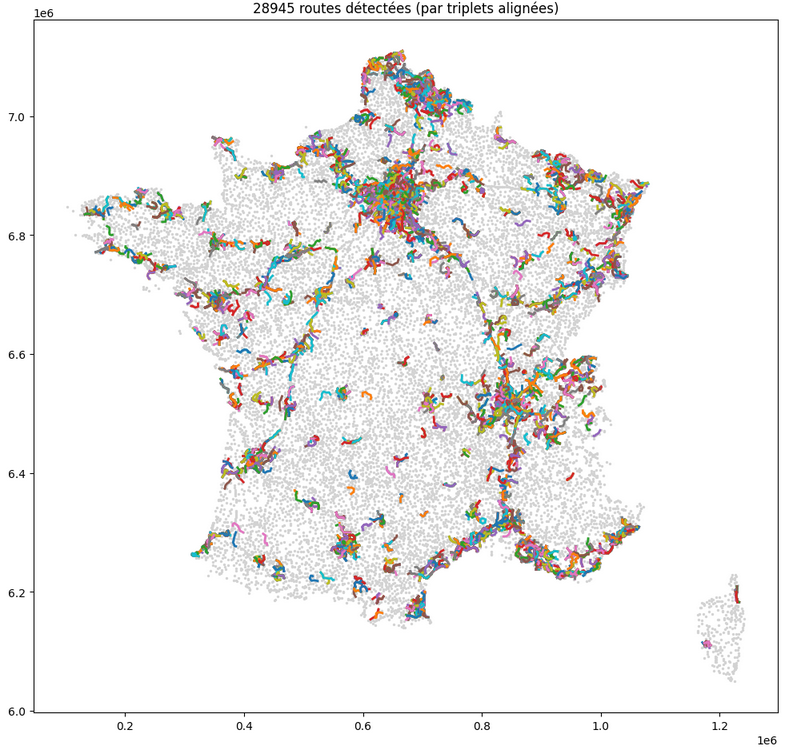
\includegraphics[width=0.55\textwidth]{Images/Res_Triplets.png}
    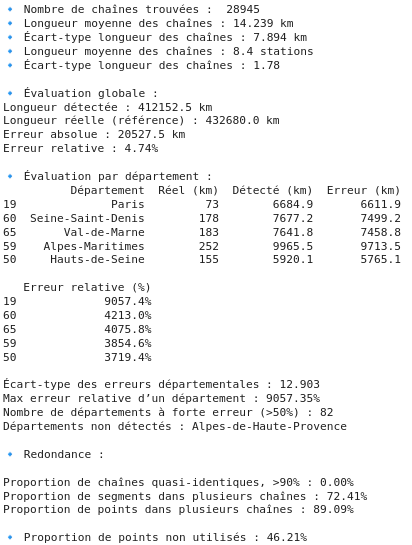
\includegraphics[width=0.5\textwidth]{Images/Metrics_Triplets.png}
    \caption{Metrics of the Triplets method}
\end{figure}

\begin{figure}[H]
    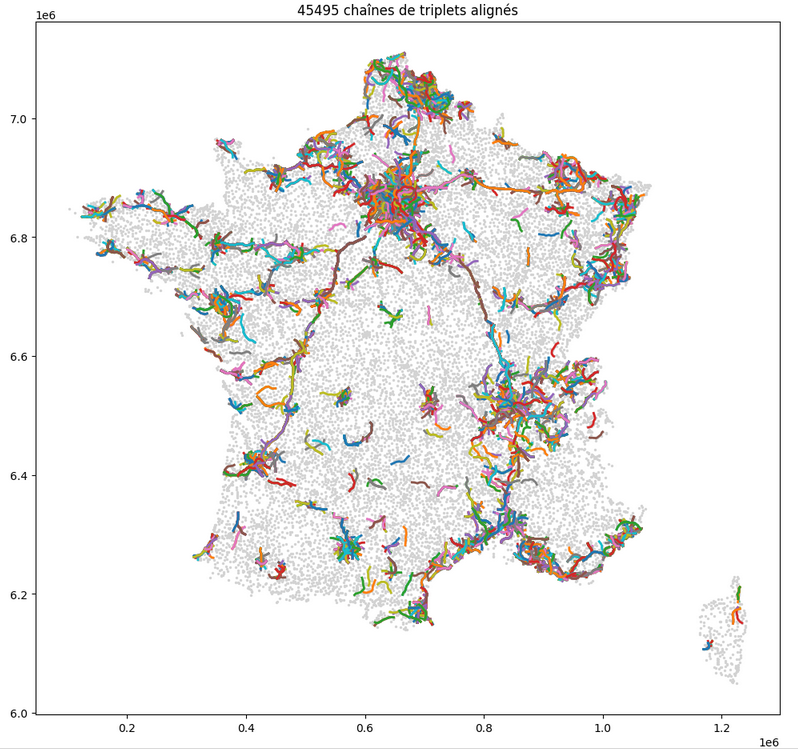
\includegraphics[width=0.55\textwidth]{Images/Res_Triplets_enhanced.png}
    \includegraphics[width=0.65\textwidth]{Images/Metrics_Triplets_enhanced.png}
    \caption{Metrics of the Enhanced Triplets method}
\end{figure}

\begin{figure}[H]
    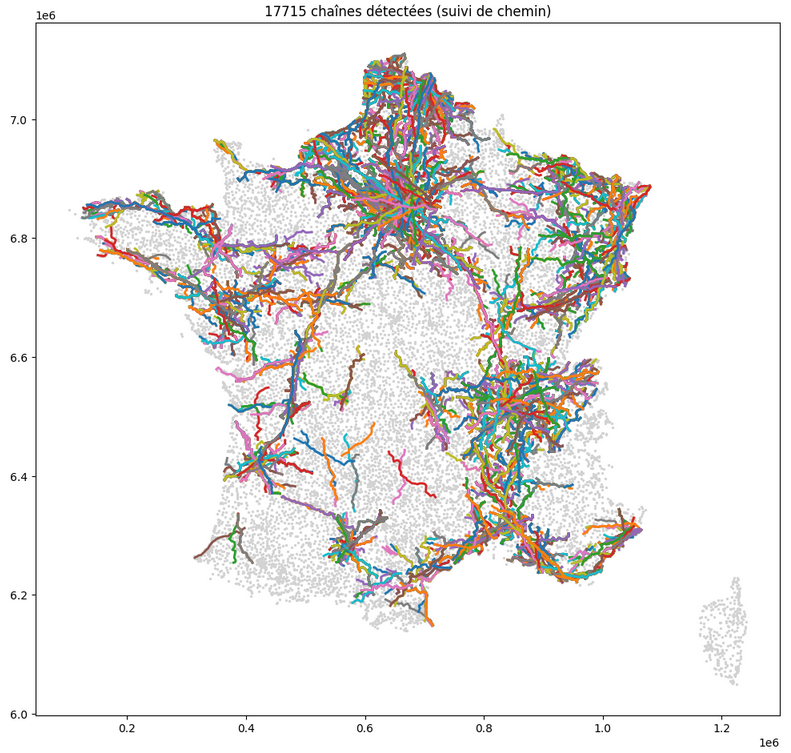
\includegraphics[width=0.55\textwidth]{Images/Res_Followline.png}
    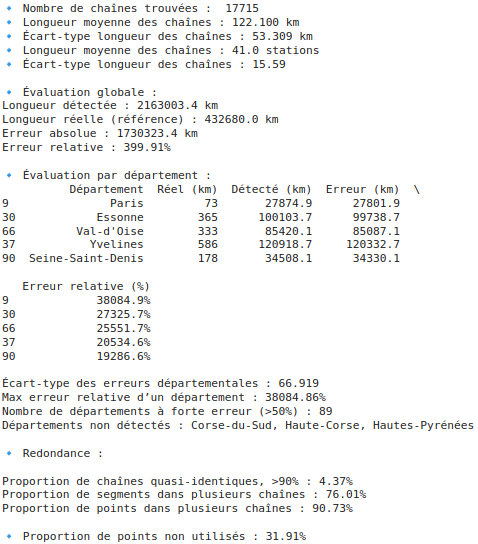
\includegraphics[width=0.5\textwidth]{Images/Metrics_Followline.png}
    \caption{Metrics of the Follow line method}
\end{figure}

\begin{figure}[H]
    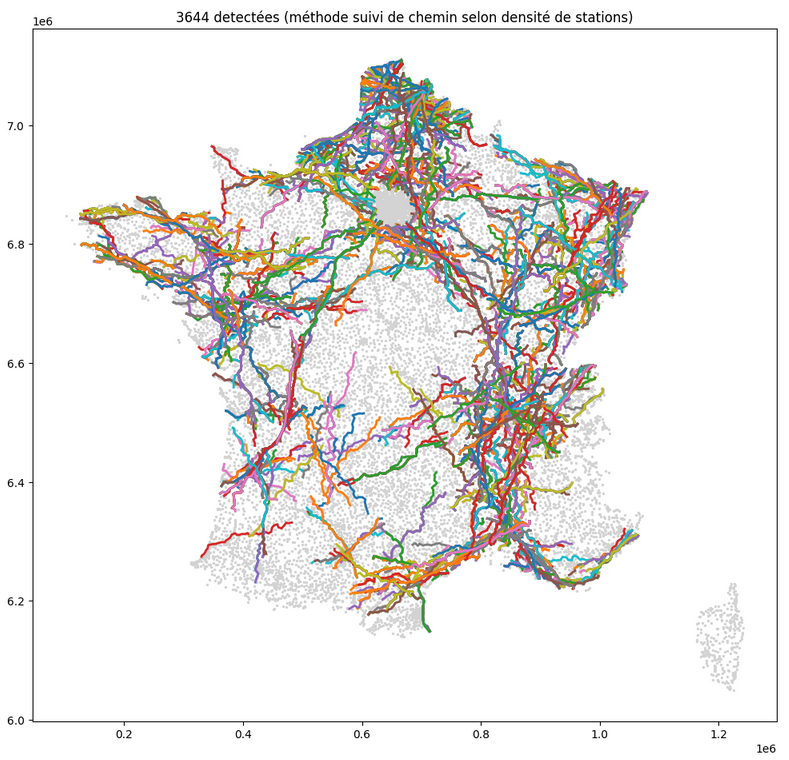
\includegraphics[width=0.5\textwidth]{Images/Res_Followline_Dens.png}
    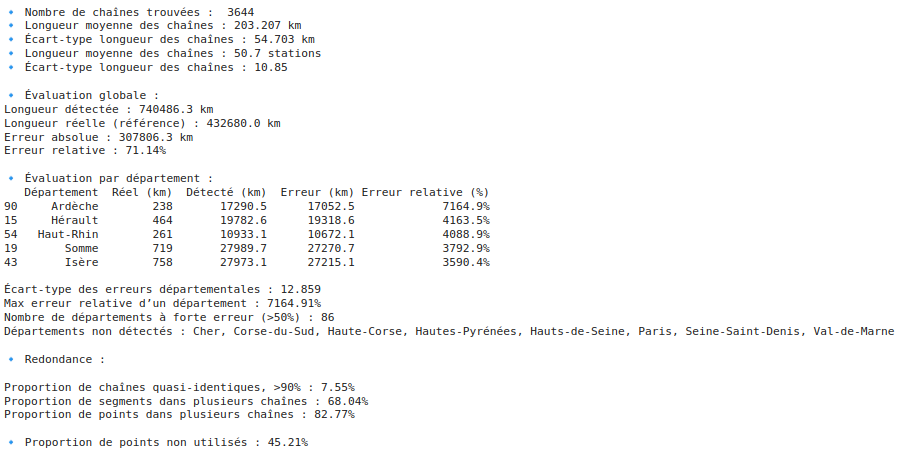
\includegraphics[width=0.8\textwidth]{Images/Metrics_Followline_Dens.png}
    \caption{Metrics of the Follow line by stations density method}
\end{figure}


\end{document}